% Chapter 4
\chapter{Straw tracking detectors} % Main chapter title
\label{Chapter4} 

The rest of this thesis will concentrate on the straw tracking detectors. This chapter will discuss the physics goals, design and operating principles of the straw tracking detectors. Chapter 6 will explain the construction and testing processes of the tracking detectors built at the University of Liverpool, which was a major part of the first two years of my PhD. Chapter 7 will discuss a beam dynamics analysis carried out using the straw tracking data. 

\section{Tracker goals and requirements}
The primary function of the straw tracking detectors is to detect the positrons from muon decays. Precise measurements of the position of the positrons and the calculated momentum allow the track to be reconstructed and extrapolated back to the muons decay point. This allows the straw tracking modules to measure the muon beam profile as a function of time throughout each fill. The data is used to determine several beam dynamics parameters of the stored muon distribution. This is required to determine the ppm corrections to the value of the muon precession frequency $\omega_{a}$ due to beam dynamics effects. The precession frequency measured is lower than the 'ideal' frequency, this is caused by muons not travelling perfectly perpendicular to the storage ring magnetic field and the momentum spread due to muons with momentum differing from the magic momentum. These effects are discussed in Chapter 7. The beam distribution must be known precisely as the muon distribution has to be convoluted with the magnetic field map in order to determine the effective field seen by the beam. There are higher order multipole terms that lead to small deviations in the effective magnetic field, affecting the muon distribution. These need to be accounted for to accurately calculate $a_{\mu}$. Therefore measuring the beam during the fills is the primary goal of the tracking detectors.

The secondary aim is to determine and minimise the systematic uncertainties on $\omega_{a}$ as determined from the calorimeter data. The tracking detectors are used to isolate short time windows in which multiple positrons hit the calorimeter. This is used to give a momentum measurement of the charged particle that can be compared with the measured energy as well as providing information on the systematic uncertainties on $\omega_{a}$. These include muon loss, calorimeter pileup and calorimeter gain \cite{Reference29}. Detected tracks are used to identify calorimeter pileup events where two (or more) particles enter a calorimeter crystal within the time resolution of the calorimeter and are counted as a single particle with the combined deposited energy. This causes lower momentum positrons, which have a different phase, to enter into the wiggle plot and if left unaccounted for results in a mis-measurement of $\omega_{a}$ on the 100 ppb level. Tracking detectors are able to reconstruct multiple tracks within the same time window, which are extrapolated to the calorimeter and as such can identify if multiple particles have hit the calorimeter crystal in this time period. 

The so called muon loss uncertainty refers to the uncertainty associated with muons that leave the storage ring before they decay. Muon loss occurs when muons with insufficient energy to be confined in the storage region leave this volume and are detected by the calorimeters. These muons typically have enough energy to travel through multiple calorimeters leading to coincidence events. Using the track momentum and the calorimeter energy these muons can be identified and the rate of muon losses can be determined, and accounted for in the $\omega_{a}$ fits. These lost muons can have a different average spin direction compared to the stored muons which will cause a deviation in the $\omega_{a}$ calculated which is evaluated using high statistics simulation.

The tertiary goal is to look for an oscillation in the vertical decay angle of the emitted positron to see if there is a tilt in the muon precession plane away from the vertical direction. This would demonstrate either a longitudinal or radial component of the storage ring magnetic field or that the muon has a non-zero permanent Electric Dipole Moment (EDM). Both effects would alter the $\omega_{a}$ measurement. The tracking detectors are unique in the experiment as the only detector that can measure the up-down asymmetry in the positron angle caused by a tilt in the muon precession plane \cite{Reference29}. With the tracking detectors and the increased statistics the experiment aims to make a improved measurement on the limit of the muon EDM by two orders of magnitude on the previous limit measured by the BNL experiment.

A table listing the goals for the systematic uncertainties measured using tracking detectors are listed below.

\begin{table}[h!]
\begin{center}
 \begin{tabular}{||c | c | c | m{5cm}||} 
 \hline
 Uncertainty & E821 value & E989 goal & Role of tracking \\ [0.5ex] 
 \hline\hline
 Magnetic field seen by muons & 0.03 ppm & 0.01 ppm
 & Measure beam profile on a fill by fill basis ensuring proper muon beam alignment \\ 
 \hline
 Beam dynamics corrections & 0.05 ppm & 0.03 ppm & Measure beam oscillation parameters as a function of time in the fill \\
 \hline
 Pileup correction & 0.08 ppm & 0.04 ppm & Isolate time windows with more than one positron hitting the calorimeter to verify calorimeter based pileup correction \\
 \hline
 Calorimeter gain stability & 0.12 ppm & 0.02 ppm & Measure positron momentum with better resolution than the calorimeter to verify calorimeter based gain measurement \\
 \hline
 Precession plane tilt & 4.4 $\mu$Rad & 0.4 $\mu$Rad & Measure up-down asymmetry in positron decay angle \\ [1ex] 
 \hline
\end{tabular}
\caption{Systematic uncertainty goals for the Muon g-2 experiment and the role of tracking required to meet these goals \cite{Reference29}.}
\label{table:1}
\end{center}
\end{table}

\section{Design}

The straw tracking stations consist of 8 identical tracking modules which are placed in close proximity to each other. There are two tracking stations situated at $180^{\circ}$ (station 1) and $270^{\circ}$ (station 2) around the storage ring. These are installed inside the vacuum chambers in order to minimise multiple scattering of particles travelling through the trackers and placed directly in front of a calorimeter. The close proximity of the tracking modules to the beam enables the reconstruction of lower momentum positrons and multiple tracking modules, separated in total by $\sim$1m, ensures that the curvature of the tracks for the momentum measurement can be accurately determined. The tracking modules are constructed from two aluminium manifolds (top and bottom manifolds) fixed in place by an aluminium flange. These are both shown in figures 5.1 and 5.2 respectively. The manifolds contain 128 identically drilled holes to hold in place 128 aluminised Mylar straws. The manifolds also contain the front-end electronics and enable the supply of gas to the straws. The straws are potted into the manifolds in four rows of 32 straws. Two adjoining rows of straws are called the V layers which are angled at $7.5^{\circ}$ from the vertical plane. The other two adjoining rows are called the U layers are angled at $-7.5^{\circ}$ from the vertical plane. An aluminium tube called a Snout connects to each manifold. The Snouts are used to connect the flange to the secondary electronics which are housed in the Flobber. The Snouts contain the flexi cables which connect to the feedthrough boards. Once the manifolds have been populated with the frontend electronics, they are sealed with a lid and vacuum greased O-ring. A picture of a completed tracking module is shown in figure 5.3. The angle of the straw layers enables the vertical height of the incoming positron tracks to be calculated. The trackers are required to measure the vertical and radial beam distributions to a high accuracy. To achieve this a resolution of approximately 100 $\mu$m per position measurement in the radial axis is required. The requirements on the vertical axis are far less stringent as there is no curvature of the tracks in the vertical direction. 

\begin{figure}[th]
\centering
\includegraphics[scale=0.8]{Figures/manifold.png}
\decoRule
\caption{Photograph of two aluminium manifolds used in the construction of a straw tracking module.}
\label{fig:manifold}
\end{figure}

\begin{figure}[th]
\centering
\includegraphics[scale=0.7]{Figures/flange.png}
\decoRule
\caption{Photograph of a flange used in the construction of a straw tracking module.}
\label{fig:flange}
\end{figure}

It was determined that since the modules will be placed in vacuum, circular straws will be used as this geometry is able to hold differential pressure even when the straw wall thickness is small. The Mylar straws are 90.6mm in length and 5mm in diameter. The straws are made up of two layers of 6${\mu}$m Mylar wound in a spiral and a 3$\mu{m}$ layer between the two of adhesive to glue them together. The straws inner wall has 500 $\mathring{A}$ aluminium overlaid with 200 $\mathring{A}$ of gold, which acts as a cathode layer. The outer layer has 500 $\mathring{A}$ of aluminium which provide additional electrostatic shielding and also helps to reduce the straws leak rate\cite{Reference29}. The modules are entirely made of non-magnetic materials. This is to ensure that the precise magnetic field is not distorted by the tracking modules. 

The design specifications require a straw resolution of at least 300 $\mu$m to enable measurement of the muon beam profile to sub-cm precision. The straw resolution has been determined to be 95 $\mu$m.

\begin{figure}[th]
\centering
\includegraphics[scale=0.5]{Figures/labeledstrawtracker.pdf}
\decoRule
\caption{A photograph of a straw tracking detector labelling its key components.}
\label{fig:labeledstrawtracker}
\end{figure}

At the centre of each straw is a 25 $\mu$m gold plated tungsten wire. These are secured in place at each end by gold plated copper pins. There are two lengths of pins as the long pins at one end are used as the electrical connection with the manifold electronics while the short pins on the other end are not. Insulating end caps are placed over the short pins to stop electrical discharge.

\section{Operating principles}

The straws in the tracking detectors behave as individual drift chambers. When positrons travel through the straw they interact with the gas molecules distributed within the straw. The positrons have enough energy such that an interaction with a gas molecule will ionise the molecule which eject one or multiple electrons. This occurs randomly as the positron passes through the straw. The interaction of the positron and the molecule is called a primary ionisation. The group of electrons that are ejected from this interaction are called a cluster, with the individual electrons called primary electrons. Further ionisation through interactions of the gas by the primary electrons will produce secondary electrons.

The drift gas mixture chosen was 50:50 Argon Ethane. This gas mixture is flowed through gas inlets in the Snouts of the module at a rate of approximately 0.1LPM, which in turn flows through the straws of the manifold. Argon was selected because it is a Noble gas. These are atoms and as such have less modes of excitation in comparison to molecules. Their main energy loss during these collisions comes from ionisation leading to the primary electrons. Ethane was chosen as it has different excitation modes compared to Argon and is used to absorb the photons produced during avalanche in order to stop the breakdown of the gas. This gas is called a quencher gas \cite{driftchamber}.

Located at the centre of the straw is the sense wire. This is held at a high voltage (HV) of 1650V and acts as an anode while the straw wall which is grounded to the manifold acts as a cathode. This leads to a strong electric field in the straw tube which is directed radially out from the wire. In the presence of the electric field between the sense wire and the straw wall the interacting particles will experience a radial force. This causes the liberated electrons to travel towards the sense wire and the gas ions to travel towards the straw wall. As the electrons travel towards the sense wire they will undergo further interactions with gas molecules producing further ionisations, which will slow down their progress towards the sense wire. The overall motion of the electrons is known as drift. The drift velocity in the straw is approximately 50 $\mu{m}/ns$. Due to the presence of a strong vertical magnetic field felt in the straws an orthogonal force is put onto the travelling electrons. This leads to them traversing in a curved path with the angle of this curvature known as the Lorentz angle.

The current signal induced on the sense wire by the travelling electrons is very small. However as the electrons travel very close to the sense wire, the electric field is strong enough to accelerate them. This leads to further interactions between the electrons and gas molecules in a short time, causing an increase in the number of liberated electrons. These will go onto ionise more gas molecules leading to an effect called avalanche multiplication which produces a rapid increase in the number of liberated electrons. The straw drift chambers are known as proportional counters. This means that the signal detected by the wire due to the avalanche is roughly proportional to the number of primary ionisations. This increase in the number of electrons gives a large enough signal to be seen over the noise threshold triggering a ‘hit’ in the readout electronics and records this as the time of the signal. 

During an avalanche, the collisions can cause excitation which leads to the release of photons from de-excitation. Photons with enough energy can travel past the avalanche volume and create further electrons from interactions with the gas. This then creates their own avalanches which leads to a breakdown of the gas. To stop this from happening a quencher gas is flowed through the straws. The experiment chose Ethane as it has multiple modes of excitation and therefore can absorb photons of different energies. The avalanche period also leads to the creation of more ions. These drift towards the cathode straw wall. This long distance movement from the avalanche volume to the straw wall induces a signal which is much larger than the signal produced in the electron avalanche. The ions possess a much larger mass and so the ions drift velocity is much slower than the electrons. This means that the signal produced by the ions is separate and much later (of the order of $\mu$s) after the electron signal. The signal induced from the ions is referred to as the ion tail. 

The signal recorded from the wire due to initial ionisations by a positron gives a signal with two pulses; an initial smaller pulse from the avalanche electrons and a much longer pulse from the ion tail. The shorter pulse from the electron avalanche triggers the front end electronics. The much larger and slower ion signal is suppressed by the electronics. This means that the electronics can cope with a high rate of signals as the larger ion signal does not mask subsequent electron avalanche signals which could occur very soon after the first.

The time that the electronics is triggered is designated as the time of the hit. For the purpose of track reconstruction the path that the positron travelled needs to be determined precisely. The hit time $t_{h}$ is determined from the time that the positron entered into the straw known as $t_{0}$ along with the time the primary ionisation electrons takes to drift from the initial interaction point to the sense wire called the drift time $t_{d}$. The hit time $t_{h}$ is calculated using the equation

\begin{equation}
t_{h} = t_{0} + t_{d}.
\end{equation}
\noindent
Therefore if $t_{0}$ is known then $t_{d}$ can be calculated. This relies on detailed knowledge of the behaviour of the charged particles in the straw gas. From $t_{d}$ the distance that the charged particle travelled through the straw (and its distance away from the wire) can be inferred. This is known as the Distance of Closest Approach (DCA), which tells us the distance the particles primary ionisation happened but not the direction in which it travelled. Instead it gives a radius of possible points where the primary ionisation has occurred called the drift circle. A diagram of a positron passing through a straw and causing primary ionisations is shown in figure 5.4. No knowledge of the vertical direction is known and so this leads to a cylinder around the wire of possible points where the primary ionisation will have occurred. To resolve this issue and determine the positrons trajectory through the tracking detectors, the cylinders from multiple straws are combined to determine the positrons path. This is the reason to have the straws orientated in two different directions, as it enables the determination of the vertical direction of the positrons trajectory. 

\begin{figure}[th]
\centering
\includegraphics[scale=0.5]{Figures/driftstraw.pdf}
\decoRule
\caption{A diagram showing primary ionisations caused by the interaction of the positron with the straw gas.  This indicates how the drift time $t_{d}$ is calculated from the hit time $t_{h}$ and the $t_{0}$ value.}
\label{fig:driftstraw}
\end{figure}
\iffalse
\begin{figure}[th]
\centering
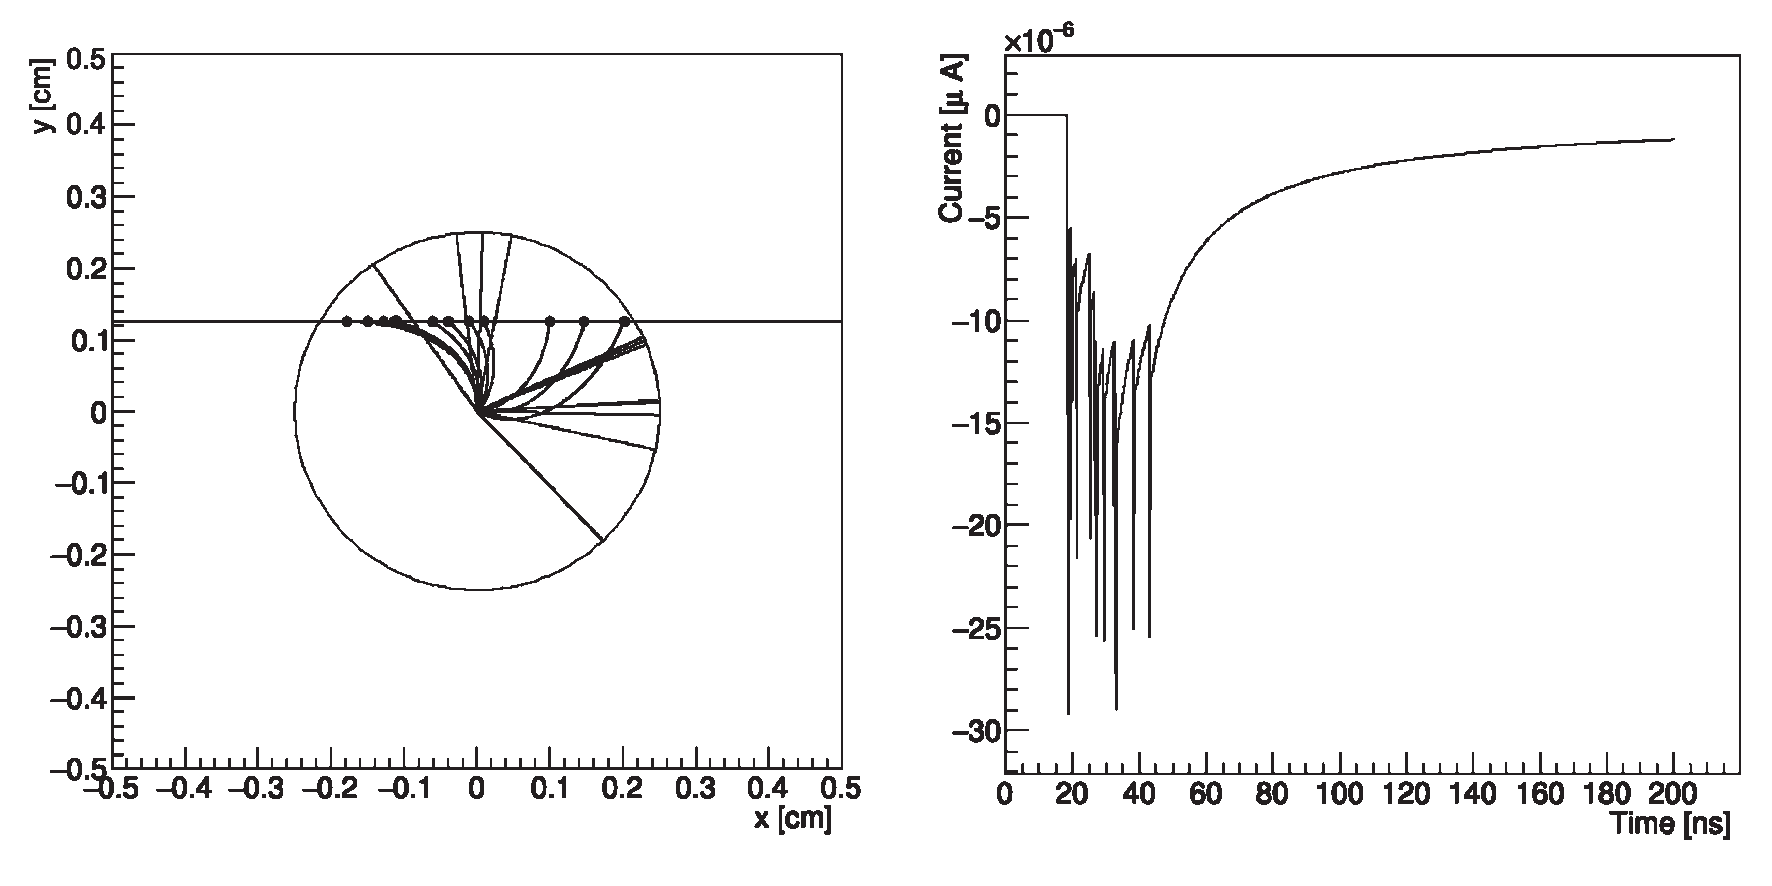
\includegraphics[scale=0.5]{Figures/StrawSignalGarfieldSim.pdf}
\decoRule
\caption{Left: Garfield simulation of the primary ionisations caused by a positron passing through the straw gas. Right: Garfield simulation of the signal measured from the sense wire for these primary ionisations.}
\label{fig:StrawSignalGarfieldSim}
\end{figure}
\fi
\section{Track formation}

The track fitting is required to work in the presence of pileup of multiple tracks at one time and include the uncertainty on the track position caused by the straw resolution. A charged particle travelling in a uniform magnetic field perpendicular to its motion will travel in a helical path. The tracking detectors are situated in the fringe field of the magnet and as such the particles experience a varying magnetic field radially and vertically. The radial field varies from 0 T at the outer end of the trackers to 0.3 T at the inner end. The vertical field also reduces to half of the 1.451 T storage ring magnetic field \cite{geanefitting}. This complicates the track fitting of the helical trajectory. This change in magnetic field will also effect the path of the charged particles as they drift through the straw, causing an added complication in obtaining the DCA for the positron. The track fitting is instead done by separating the path into short sections. 

Drift circles are created and centered around the wire, using the drift radius calculated from the drift time and the drift velocity. By comparing the neighbouring straw drift circles potential tangents can be found. To do this a line of best fit can be drawn from the shortest distance of each tangent between two drift circles.

The trajectory of the positrons path through the straw tracking detectors is calculated from the DCA of the positrons path through multiple straws, along with detailed information on the positions and orientations of the straws. The stages of track finding are as follows. For each tracking module the straw hits within a time period are grouped together. This time period is approximately 100 ns and these hits are grouped together to form a time island. Next there is spacial grouping of these hits. This is first done by grouping straw hits within the same view (U or V) in different layers if they are adjacent. These are referred to as clusters. The clusters for the U and V views for a single module are then group together to form seeds. The candidate positron tracks are formed by grouping together seeds in different modules based on which seeds are close in time and proximity to the previous one. Once straws have been identified as part of a potential track the $t_{d}$ is determined in order to calculate the drift distance for each straw. The simplified version in which a positron is travelling at normal incidence, a t0 value for a cluster with individual hit times of $t_A$ and $t_B$ is calculated using the equation

\begin{equation}
t_{0} = \frac{1}{2}((t_{A} + t_{B})-(d/v_{drift})),
\end{equation}
where d is the distance between the two wires and $v_{drift}$ is the drift velocity.

This allows a $t_{0}$ value to be calculated for each straw and hence the $t_{d}$ can be calculated in order to determine the DCA and then the drift cylinder of the positrons trajectory. This also allows the calculation of which side the positron came from which cannot be determined from a single straw. In order to determine the vertical direction the next cluster (with a different view) must be included, as these straws are orientated at a different angle. However this leads to a degeneracy when allowing for incident particles coming from any angle. The radial degeneracy of the DCA measurement means it is hard to determine which side of the wire the particle travelled, this is called the left-right ambiguity. Multiple track fitting is required to determine which set of left-right combinations gives the best fit. 

The track fitting is carried out using the GEANE (Geometry and Error Propagation) fitting algorithm \cite{geane}. This algorithm is configured to look up the field at small intervals throughout its path length to account for the varying magnetic field throughout the tracker module. The track fitting relies on only the hit information from the U or V layers. This fitting algorithm connects the DCA's determined in each of the straws it passed through in the tracking station. One can define a $\chi^{2}$ for a track by dividing the residuals of measured and predicted track parameters by their errors:

\begin{equation}
\chi^{2}= (\vec{p}-\vec{x})^{T}(\sigma^{-1})(\vec{p}-\vec{x}),
\end{equation}
\noindent
where $\vec{p}$ are the predicted track parameters given from the fit, $\vec{x}$ are the measured track parameters and $\sigma$ is the covariance matrix x of errors on the fitted parameters.

The Geant4 error propagation calculates the error matrices and predicted track parameters by starting off with guesses and then propagating the track parameters from these guesses. This is done by propagating the positrons by their average trajectories and splitting the steps into small enough sections. Meaning that a helical trajectory can be used in a magnetic field with a very small variation. Minimising the $\chi^{2}$ with respect to the track parameters leads to an improvement in the track fit \cite{geanefitting}. An example of a formed track candidate is shown in figure 5.5.

\begin{figure}[th]
\centering
\includegraphics[scale=1.4]{Figures/Track.png}
\decoRule
\caption{A plot showing an example of a track candidate.}
\label{fig:Track}
\end{figure}

\section{Track extrapolation}

The track parameters can be extrapolated back to the muon decay point or forwards to the calorimeter. The track information determined at its entry point into the tracking station is used in the extrapolation algorithm. This propagates the particles trajectory from the station entry point backwards through the changing magnetic field to the estimated muon decay position in the storage region. This information is used to observe the stored muon beam profile. This is problematic as there is no constant decay position and so this point has to be predicted by the extrapolation algorithm. This is taken to be the position of radial tangency, where the positrons momentum is tangential to the storage rings magic radius. 

The straw tracker station is situated directly upstream of a calorimeter to be able to extrapolate the tracks downstream to the calorimeter. The extrapolation downstream is used to estimate its hit position in the calorimeter. This can then be compared to what the calorimeter detected and act as a cross check between the two detectors. The data can also be used to determine if the two detectors are aligned correctly and also reduce pileup of hits detected in the calorimeter. Pileup is caused if two low energy positrons hit the same calorimeter crystal within its timing and spacial resolution and are counted as one high energy positron.

The extrapolation algorithm uses a Runge-Kutta Nystrom algorithm \cite{rungekutta1}\cite{rungekutta2}. 
This uses track parameters determined for the entry point and exit point of the tracking station to either extrapolate forwards to the calorimeters or backwards to the decay point. This must also take into account the changing magnetic field that is seen in the tracking station region (fringe field region) and the varying magnetic field to the muon storage region. This extrapolation is done in small steps in order to determine the magnetic field at each location of the particles trajectory and if the particle is likely to hit material. If this is the case then the particle will scatter, losing energy and altering its path. These particles will not be used in the precise analyses of the beam dynamics.

\section{Tracking quality cuts}

Quality cuts are applied to the data in order to reduce the tails observed in the tracking distributions and reduce the tracking uncertainties. Since the tracking detectors are not the primary detectors for this experiment, the track quality cuts were chosen to be fairly strict. They are optimised such that a small subset of tracks, representative of the whole sample, are as accurate as possible. This will need to be improved for track only analyses of the g-2 data (for example the EDM measurement), but is sufficient for the primary goal of measuring the beam dynamics. Effective quality cuts include having at least 12 straw hits required per track as a low number of hits leads to an increased error in determining the vertex position, removing tracks which have from start to finish more than 30$\%$ of layers without a hit, requiring that the track residual (measured - predicted) position is smaller than 0.5mm for any hit. Below in Table 5.2 is a summary of the quality cuts used in the tracking analysis.

\begin{table}[h!]
\begin{center}
 \begin{tabular}{||c | m{5cm}||} 
 \hline
 Parameter & Quality Cut \\ [0.5ex] 
 \hline\hline
 Non-failed track/vertex &  \\ 
 \hline
 No volumes hit & \\
 \hline
 Number of straw hits  & >= 12 \\ 
 \hline
 pValue & 5$\%$ \\ 
 \hline
 $\sigma_{y}$ and $\sigma_{r}$ & 0.5 < $\sigma_{y}$ 3.5 mm and 0.5 < $\sigma_{r}$ 5.0 mm\\
 \hline
 Track Entrance Point (at 1st module) & 60 < x < 150 mm and -40 < y < 40 mm \\
 \hline
Drift times & 0 < and < 70 ns \\ 
 \hline
 Track residuals & < 500 $\mu$m \\
 \hline
 Fraction of missed layers & < 30$\%$ \\ 
 \hline
 |U - V hits| & <= 4 \\ [1ex] 
 \hline
\end{tabular}
\caption{The quality cuts applied to the tracking detector data.}
\label{table:2}
\end{center}
\end{table}

\section{Readout electronics}

Once a signal has been produced on a sense wire two sets of electronics are used to convert the analog signal into a digital signal. These are the frontend electronics and the backend electronics. The frontend electronics are the boards which detect the wire signals and processes these into straw hits. A photograph of the frontend electronics is shown in figure 5.6. The backend electronics are the electronic boards used to interface the data from all the frontend boards and also synchronise the signals using the experimental clock information.

\subsection{Frontend electronics}

\begin{figure}[th]
\centering
\includegraphics[scale=0.4]{Figures/manifoldelectronics.pdf}
\decoRule
\caption{A photograph of the manifold frontend electronics showing the important components.}
\label{fig:manifoldelectronics}
\end{figure}

The frontend electronics consist of ASDQs (Amplifier Shaper Discriminator with charge (Q)) boards which are located inside the tracker manifolds and used to convert the analog signals from the sense wire to digital hits. This data is then sent to the TDC (Time to Digital Converter) boards which are contained in the box attached to the Snouts called the Frontend Low voltage Optical Box to BackEnd Readout (FLOBBER). The ASDQ boards are situated directly at the end of the sense wire and as such are the first electronics to process the wire signal. The ASDQ boards are connected directly into the manifolds via long pins to provide electrical connection, with every ASDQ boards connecting to 16 sense wires and so requires four ASDQ boards per manifold.

The ASDQ boards take several steps in converting the analog signal into a digital signal. These are amplification, signal shaping, baseline restoration and discrimination. The signal is shaped to smooth out the multiple small peaks that are created by the multiple primary ionisations produced by the charged particle travelling through the straw. This creates a single smooth peak for a single charged particle. Baseline restoration is used to remove the long signal tail that arises from the much slower ion signal. Doing this also ensures that primary ionisations from the next charged particle to pass through the straw are not consealed by the ion tail. Meaning the two signals can be easily distinguished, increasing the rate of signals that can be determined. The discriminator is used to register when the signal passes a threshold and recording the digital straw hit as being from the leading edge where the signal first crosses over the threshold to the trailing edge where the signal goes below the threshold. A diagram showing the step the ASDQ takes to convert the analog to digital signal is shown in figure 5.7.

\begin{figure}[th]
\centering
\includegraphics[scale=0.5]{Figures/asdqsignalpath.png}
\decoRule
\caption{A diagram displaying the steps the ASDQ carries out to convert an analog signal to a digital signal. (a) Multiple short signals are measured for each of the avalanches caused the the primary interactions of the positron with the straw gas. (b) The amplification and shaping of the short signals into one smooth signal. (c) The discriminator selects the data that passes above the threshold shown by the red line. The blue lines indicate the section of the signal that passes above this threshold. (d) The digital signal created for the leading and trailing edges of the smoothed out signal. The ion tail is not included in the diagram \cite{analogtodigital}}.
\label{fig:asdqsignalpath}
\end{figure}

The digital signals from the ASDQ boards are then sent to a TDC motherboard via flexicables. A straw tracking module contains two logic boards and four TDC motherboards. With each motherboard containing two TDC chips each of which connects to an ASDQ board. The electronics for the U layer is housed in the bottom manifold and the electronics for the V layer in the top manifold. The ASDQ digital signal information is carried via Low Voltage Digital Signal (LVDS) flexicable to a TDC board which is stored in the FLOBBER and holds the HV and logic boards (LB). The FLOBBER was designed to hold the electronics externally (outside the vacumm chamber) from the manifold as they do not need to be directly connected to the sense wires and makes it much easier to cool and gain access to these electronics. The TDC board time stamps the ASDQ signal to the precision of 625 ps by the use of the experiments 40 MHz clock. This information is sent to the backend electronics including the hit channel and time of the signal leading edge which is set as the hit time. The low and high voltage required for the tracking modules is supplied by a low voltage crate and a high voltage CAEN SY127 crate \cite{CAEN} located in a rack in the centre of the storage ring. 

\begin{figure}[th]
\centering
\includegraphics{Figures/daqdata}
\decoRule
\caption{The path of the straw hit data, clock and control signals through the frontend and backend electronics in the straw tracker readout system.}
\label{fig:daqdata}
\end{figure}

\begin{figure}[th]
\centering
\includegraphics[scale=0.8]{Figures/daqdatachain}
\decoRule
\caption{The hierarchy of frontend and backend boards and the numbers of each electronic boards used in the straw tracker readout system.}
\label{fig:daqdatachain}
\end{figure}

\subsection{Backend electronics}

The backend electronics include logic boards (LB), the FC7 and the AMC13. The two LBs per module are also located in the FLOBBER and provide an interface to the ASDQ-TDC pairs (1 LB per 4 pairs) used to supply clock and control signals to the TDC's and gather the information together into a single data block to be processed downstream in the FC7 and AMC13 boards. The LB consists of three external interfaces. A fibre-optic cable which connects to the higher level backend electronics to receive the external clock and control signals, the LV line supplying low voltage to the frontend electronic boards and a serial communication port to the slow control hardware. The fiber optic cables are required to send data over large distances very quickly and so the higher level backend electronics can be stored away from the trackers. These are placed in the centre of the ring away from the magnetic field storage region, allowing magnetic materials to be used.

Three FC7 $\mu$TCA advanced mezzanine cards (AMC) are located in the $\mu$TCA crate located at the centre of the storage ring, each connected to 16 LBs (one tracker stations worth). The FC7 is used to supply the clock and control signals for the LBs and collect a hit data block from all the LBs into a singular block using an event builder. The AMC13 board is the most downstream board which is also housed in the $\mu$TCA crate and collects together the hit data from the 3 FC7 boards as well as distributing the clock and control signals to the tracker modules. The AMC13 connects to a computer in the counting room via a Gigabit Ethernet (GbE) fiber in which the hit data blocks from the frontend boards can be saved to disk. Diagrams of the heirachy of the frontend and backend electronics are shown in figures 5.8 and 5.9.

\section{Choice of wire voltage}

Gain measurements were carried out to find the optimal operational wire voltage for the modules. The gain is the ratio of the final number of electrons detected by the straw wire to the number of electrons initially liberated in a gas. A high voltage on the straw wire will lead to a larger electric field strength and therefore electrons in the straw will have higher energies after collisions, leading to an increased likelihood of more ionisations. Therefore a larger signal is detected by the straw wire. However if the wire voltage is set too high the gas in the straw starts to breakdown with too many hits being detected by the wire. This amplifies the measurement of one charged particle leading to saturation of the electronics. If the voltage is too low, it will give a low electric field strength in the straw. Thus too few electrons will be liberated during collisions to produce a large enough signal in the wire. As the signal must be above the discriminator threshold of 200 mV, this would lead to loss of data recorded.

An optimal wire voltage must be found in between these two effects. This is the plateau region, where the best balance of high gas gain along with the minimum breakdown of gas is located. To determine the optimal wire voltage, the number of straw hits for various wire voltages was measured. This was carried out using a radioactive $Sr^{90}$ $\beta^-$ decay source with two types of gases; 80:20 $Ar:C0_{2}$ and 50:50 $Ar:C_{2}H_{6}$. As can be seen by figure 5.10 for the tracker straw gas using 50:50 $Ar:C_{2}H_{6}$ below 1200 V the gain is too low for straw events. With increasing voltage the gain increases and so does the number of hits recorded by the electronics. At a voltage of approximately 1550 V the number of hits recorded plateaus. This indicates that at this voltage approximately all of the beta particles travelling through the straw are detected by the wire as hits. This continues until the voltage reaches about 1700V. From there onwards the hit rate increases due to an increasing gain indicating the breakdown of the gas. This means that each beta particle will cause multiple hits to be recorded. Therefore the optimal voltage for the wire should lie on this plateau range, with a voltage of 1650V being chosen.

\begin{figure}[th]
\centering
\includegraphics[scale=0.8]{Figures/plateau}
\decoRule
\caption{A plateau scan plot showing the number of hits from a $Sr^{90}$ source with wire voltage for both 50:50 $Ar:C_{2}H_{6}$ and 80:20 $Ar:C0_{2}$. This shows that for $Ar:C_{2}H_{6}$ the plateau region is in the range of approximately 1550V - 1700V. Therefore the ideal wire voltage is within this range.}
\label{fig:plateau}
\end{figure}

\section{Data quality monitoring}

Data Quality Monitoring (DQM) is used to enable the monitoring of the tracking detectors performance in real time during data taking. This is used to monitor the trackers performance and looking for problems with the data that shifters can quickly identify and rectify. Examples of things that can be monitored in real time include the position and motion of the extrapolated beam, the number of hits per straw which is used to look for noisy or dead straw and any change in the drift time which could indicate a leak in the straw. The tracking detectors have performed extremely well during data taking periods and so far there has been no detector down time due to HV trips. 

The control of data aquisition (DAQ) for the experiment is controlled by the Maximally Integrated Data Acquisition System (MIDAS) software package. This is used to handle data from the frontend electronics, building events coming from various hardware/software locations and writing the data. This converts MIDAS data to ART data (the event processing framework used for the experiment) and allows for real time viewing of data taking via a web page. figures 5.11 - 5.13 show several tracking detector DQM web pages.

\begin{figure}[th]
\centering
\includegraphics[scale=0.3]{Figures/DQMoverview.jpeg}
\decoRule
\caption{A DQM page displaying tracking plots during data taking. Top right: showing the number of straw hits in both stations and each tracker module. Bottom right: The expected and measured straw hit drift time. Bottom left: The average number of hits per TDC for the last 20 events for both stations. Top left: Unpacking information.}
\label{fig:DQMoverview}
\end{figure}

\begin{figure}[th]
\centering
\includegraphics[scale=0.3]{Figures/DQMtracks.jpeg}
\decoRule
\caption{A DQM page showing near real time track candidates for 3 modules in station 1.}
\label{fig:DQMtracks}
\end{figure}

\begin{figure}[th]
\centering
\includegraphics[scale=0.3]{Figures/DQMhits.jpeg}
\decoRule
\caption{A DQM page displaying the number of hits in almost real time for the front two tracking modules of station 1.}
\label{fig:DQMhits}
\end{figure}

\section{Straw Tracker performance}

The data taking for the run 1 physics was during 23rd March - 7th July 2018. These tracking plots in figures 5.14 - 5.21 were created using a dataset during this run called the 60 hour data set which was taken during 19th - 23rd April 2018. 

Figure 5.14 shows the all straws hits in both stations and is the first plot looked at to determine if there are any problems with the straws. This includes checking that there are no dead channels and no stand out straws with substantially more hits, which indicates a noisy channel.

\begin{figure}[th]
\centering
\includegraphics[scale=0.5]{Figures/DigitChannelMap_.png}
\decoRule
\caption{A 3D graph displaying the number of hits in each straw for both tracking stations. The higher numbered straws are positioned closer to the storage ring and so more hits are recorded.}
\label{fig:DigitChannelMap_}
\end{figure}

Figure 5.15 displays the sum of all the drift times for each straw. The hit time for the straw is used to group straw hits together to form tracks. From this a $t_0$ value can be determined and using equation 5.1 the drift time is calculated.

\begin{figure}[th]
\centering
\includegraphics[scale=0.4]{Figures/StrawDriftTime_.png}
\decoRule
\caption{The straw drift time as measured during data taking by the tracking detectors.}
\label{fig:StrawDriftTime_}
\end{figure}

Figure 5.16 shows the track moment for all tracks. It is not a smooth peak as it includes certain regions where they cross over the thresholds of the quality cuts. Figure 5.17 displays the extrapolated tracks positions in the storage ring. Figure 5.18 shows the azimuthal muon beam spot.

\begin{figure}[th]
\centering
\includegraphics[scale=0.4]{Figures/hMomentum_.png}
\decoRule
\caption{The track momentum distribution measured for tracks by the tracking detectors.}
\label{fig:hMomentum_}
\end{figure}

\begin{figure}[th]
\centering
\includegraphics[scale=0.9]{Figures/trackextrap.png}
\decoRule
\caption{A top-down view of of the storage ring with the positions of the two tracking stations and the reconstructed decay positions of the positron tracks.}
\label{fig:trackextrap}
\end{figure}

\begin{figure}[th]
\centering
\includegraphics{Figures/beamposition.png}
\decoRule
\caption{The muon beam distribution reconstructed from all extrapolated tracks}
\label{fig:beamposition}
\end{figure}

Figure 5.19 is the radial position versus time of the tracks showing the coherent betatron oscillation of the stored muon beam. The radial position of the tracks is shown in figure 5.20. From this plot the radial distribution looks like its peak is at around 20 mm. However if you look at figure 5.19 you can see that the distribution bunches up around this value and the projection of this onto the x axis is what is displayed in figure 5.20. If you look at the CBO it can been seen that the peak is actually around 9 mm. The vertical position of the tracks is shown in figure 5.21 for completeness.

\begin{figure}[th]
\centering
\includegraphics[scale=0.9]{Figures/trackercbo.png}
\decoRule
\caption{The track reconstructed decay radial position versus time for all tracks measured by the tracking detectors.}
\label{fig:trackercbo}
\end{figure}

\begin{figure}[th]
\centering
\includegraphics[scale=0.4]{Figures/RadialPosition_.png}
\decoRule
\caption{Reconstructed decay radial position for measured tracks.}
\label{fig:RadialPosition_}
\end{figure}

\begin{figure}[th]
\centering
\includegraphics[scale=0.4]{Figures/VerticalPosition_.png}
\decoRule
\caption{Reconstructed decay vertical position for measured tracks.}
\label{fig:VerticalPosition_}
\end{figure}

More details of the beam dynamics results will be given in chapter 7. The following chapter will provide details on the construction of the straw tracking modules. These results would not be possible if the tracking detectors were not made to very high specifications, which the following chapter will discuss in detail.



